% !TeX program = lualatex
% !TeX root = luaking.tex
% !TeX encoding = UTF-8
% !TeX spellcheck = cs_CZ
%---------------------------------------------------------------------------------------------------
% file spojity_model_elmag_p.tex
\graphicspath{{../src/TEO/img/}}
%==============================Kapitola: Spojité matematické modely jednotlivých polí ==============
\setchaptertoc
\chapter{Spojité matematické modely polí}

  \section{Elektromagnetické pole}
    \subsection{Veličiny elektromagnetického pole a jejich jednotky}
      \fbox{Elektrický náboj} je \emph{skalární veličinou}. Jednotkou je \emph{coulomb [C]}. Má
         kvantový charakter (tj. je roven celistvému násobku elementárního náboje $e =
         1,602\cdot10^{-19}C$), avšak v technických aplikacích k tomu nepřihlížíme. Náboj $Q$
         může být rozložen:
         \begin{itemize}[noitemsep]
            \item \emph{prostorově} v objemu $V$ s objemovou hustotou
               \begin{equation}\label{TEMP:eq_q_varrho}
                  \varrho = \frac{dQ}{dV} \quad [C\cdot m^{-3}]
               \end{equation}               
            \item \emph{plošně} na ploše $S$, s plošnou hustotou
               \begin{equation}\label{TEMP:eq_q_sigma}
                  \sigma = \frac{dQ}{dS} \quad [C\cdot m^{-2}]
               \end{equation}                 
            \item \emph{lineárně} na křivce $l$, s lineární hustotou
               \begin{equation}\label{TEMP:eq_q_tau}
                  \tau = \frac{dQ}{dl} \quad [C\cdot m^{-1}]
               \end{equation}                 
         \end{itemize}
         Rozlišujeme:
           \begin{itemize}[noitemsep]
             \item \textbf{volné náboje}: mohou se přemisťovat v makroskopických
             vzdálenostech,
             \item \textbf{vázané náboje}: mohou se přemisťovat jen v
             mikroskopických vzdálenostech.
           \end{itemize}
         Volnými náboji jsou volné elektrony v kovech nebo ionty v elektrolytech (jsou odpoutány od
         atomů, resp. molekul a volně se mezi nimi pohybují); vázané náboje vznikají polarizací
         dielektrika.
         
      \vspace{1em}
      \fbox{Elektrický proud}\label{TEMP:kap_el_proud_velicina} je znám z každodenního života,
        přesto je velmi důležité umět tento pojem vnímat jak pro označení „jevu“ (kap.
        \ref{TEMP:kap_elproud_jev}), tak jako fyzikální veličinu, která tento jev kvantitativně
        popisuje (kap. \ref{TEMP:kap_el_proud_velicina} ). Elektrický proud je \emph{skalární
        fyzikální veličina} tzn. $I$ resp. $i$, jejíž jednotkou je základní jednotka soustavy SI:
        \emph{ampér} - [A]. V této soustavě jednotek je ampér definován na základě silových
        účinků mezi dvěma vodiči, kterými prochází elektrický proud. Tato síla je magnetického
        původu, avšak magnetické pole vzniká jako důsledek pohybu elektrického náboje. Je tvořen
        uspořádaným pohybem elektrických nábojů.
        
        Připojíme-li vodič ke zdroji elektrického napětí, elektrické pole uvnitř působí elektrickou
        silou na vodivostní elektrony, vyvolává jejich pohyb a tím vytváří elektrický proud, který
        je po krátké době \emph{stacionární} (ustálený, nezávislý na čase). Jestliže vodičem projde
        náboj $\Delta Q$ resp. $dQ$ za časový interval $\Delta t$ resp. $dt$, lze definovat
        \emph{průměrný} resp. \emph{okamžitý} proud ve vodiči:
        \begin{itemize}[noitemsep]
          \item \textbf{průměrný} elektrický proud: $$I_{AV} = \frac{\Delta Q}{\Delta t}
                \quad[A],$$
          \item \textbf{okamžitý} elektrický proud (který je limitním případem proudu průměrného,
                studujeme-li množství náboje, které projde průřezem vodiče za infinitezimální
                (nekonečně krátký) časový interval): $$i = \lim_{\Delta t \rightarrow 0}\frac{\Delta
                Q}{\Delta t} = \frac{dQ}{dt} \quad[A].$$ V ustáleném stavu protéká všemi průřezy
                vodiče stejně velký proud,
          \item speciálně pohybuje-li se náboj vodičem rovnoměrně, nazýváme proud
                \textbf{stejno\-směr\-ným}, $I(t) = \text{konst}$, a platí $$ I_{DC} =
                \frac{Q}{t}\quad[A] $$
        \end{itemize}        

        Elektrický proud jako \emph{jev} charakterizuje jednu z forem fyzikálního pohybu, kterou je
        \textbf{uspořádaný pohyb elektricky nabitých částic} v látce. Přestože jakýkoliv elektrický
        proud je vždy tvořen pohybujícími se náboji, nemusí všechny pohybující se náboje vytvářet
        elektrický proud. Ve vodiči dochází ke vzniku trvalého elektrického proudu za těchto
        podmínek:
          \begin{itemize}[noitemsep]
            \item vodič se musí nacházet v trvalém elektrickém poli, což je realizováno pomocí tzv.
                  \emph{zdroje} (generátoru) elektrického napětí,
            \item ve vodiči musí být přítomny volné nosiče elektrického náboje.
          \end{itemize}
        
        Podle charakteru vnějšího elektrického pole lze rozlišit tři základní druhy proudů:
          \begin{description}[noitemsep]
            \item\textbf{stejnosměrný} proud vzniká tehdy, jestliže má intenzita elektrického pole
                   konstantní orientaci,
            \item\textbf{střídavý} proud ve vodiči vytváří vnější elektrické pole, jehož intenzita
                  periodicky mění svou orientaci na opačnou,
            \item\textbf{stacionární} stejnosměrný proud vzniká ve vodiči, je-li intenzita
                  elektrického pole konstantní co do velikosti, směru i orientace.
          \end{description}  

       Nabité částice představující volný náboj ve vodičích jsou v neustálém chaotickém tepelném
       pohybu (viz molekulová fyzika a termodynamika). Jedná se o \emph{mikroskopický pohyb}, který
       nemá za následek makroskopicky pozorovatelné přemístění náboje. Pokud ve vodiči vytvoříme
       elektrické pole, tepelný pohyb nabitých částic neustane, ale k náhodné složce rychlosti
       přibude ještě složka rychlosti ve směru vloženého pole.
       
       Při studiu elektrického proudu v kovových vodičích se zabýváme ustálenými proudy
       vodivostních elektronů, které v kovu vytváří tzv. \emph{elektronový plyn}. Tyto vodivostní
       elektrony jsou téměř volné a pohybují se v poli kladných iontů uspořádaných v krystalové
       mřížce.
        
       Experimentálně lze elektromagnetické pole prokázat silovým působením na elektricky nabité
       částice (kapitola \ref{fyz:IIchapI}). Celkovou sílu $\vec{F}$ lze rozložit na elektrickou 
       sílu $\vec{F}_e$, nezávislou na tom, zda je nabitá částice v klidu nebo v pohybu vůči 
       vztažné soustavě a na magnetickou sílu $\vec{F}_m$, působící jen na pohybující se částice. 
       Elektromagnetické pole má tedy dvě složky: \textbf{elektrické pole}, působící na náboj silou 
       $\vec{F}_e$ a \textbf{magnetické pole}, působící na pohybující se náboj silou $\vec{F}_m$  
       \cite[s.~13]{Mayer2001}. 
      
      \vspace{1em}
      \fbox{Intenzita elektrického pole $\vec{E}$} je vektorovou veličinou charakterizující
        \emph{elektrické pole}.
        Je definována jako 
        \emph{síla působící na nepohybující se jednotkový bodový náboj}:
        \begin{equation}\label{TEMP:eq_E}
          \vec{E} = \frac{\vec{F}_e}{Q} \quad\left[\frac{V}{m}\right]  
        \end{equation}        
        kde $\vec{F}_e$ je elektrická síla působící na náboj $Q$.
      
      \vspace{1em}
      \fbox{Magnetická indukce $\vec{B}$} je vektorovou veličinou charakterizující \emph{magnetické
        pole}. Je definovována vztahem
        \begin{equation}\label{TEMP:eq_B}
          \vec{F}_m = Q(\vec{v}\times\vec{B}) \quad[T]  
        \end{equation}        
        kde $\vec{F}_m$ je magnetická síla působící na náboj $Q$ pohybující se rychlostí $\vec{v}$.
        Jednotkou je \emph{tesla} $[T]$.
    
        Síla, jež působí elektromagnetické pole na pohybující se náboj se nazývá \textbf{Lorentzova
        síla}
        \begin{equation}\label{TEMP:eq_Lorentz}
          \vec{F} = \vec{F}_e + \vec{F}_m =Q(\vec{E} + \vec{v}\times\vec{B}) \quad[N]  
        \end{equation}        

    \subsection{Maxwellovy rovnice}
      Makroskopická teorie elektromagnetického pole v klasickém pojetí vychází ze základních zákonů
      vyjádřených \emph{Maxwellovými rovnicemi (MR)}. Lze je zapsat buď v \textbf{integrálním} (viz 
      kap. \ref{fyz:IIchapIII}), nebo \textbf{diferenciálním tvaru} (viz kap. \ref{fyz:IIchapII}). 
      V integrálním tvaru popisují elektromagnetické pole v jisté prostorové oblasti $\Omega$, 
      kdežto v diferenciálním tvaru ve vnitřním bodě této oblasti. Soustavu vlastních MR 
      představují první čtyři páry rovnic; často se k nim připojuje jako další základní rovnice 
      elektromagnetického pole rovnice kontinuity pro vodivý proud. Její integrální a diferenciální 
      tvar reprezentují poslední dvě rovnice.
      \begin{subequations}
        \begin{alignat}{3}
          \oint_{\mathcal{C}}\vec{H} \dd{\vec{l}}, &= I+\der{\Psi}{t}
                                       \quad &&\rot{H}&&=\vec{J}+\pder{\vec{D}}{t}             \\
          \oint_{\mathcal{C}}\vec{E} \dd{\vec{l}}, &= -\der{\Phi}{t}
                                       \quad &&\rot{E}&&=-\pder{\vec{B}}{t}                    \\
           \int_{\mathcal{S}}\vec{D} \dd{\vec{S}}, &= Q \quad\quad\;   
                                       \quad &&\diver{D} &&=\rho_V                             \\
           \int_{\mathcal{S}}\vec{B} \dd{\vec{S}}, &= 0 \quad
                                       \quad &&\diver{B}&& =0                                  \\
           \int_{\mathcal{S}}\vec{J} \dd{\vec{S}}, &= -\der{Q}{t} 
                                       \quad &&\diver{J}&&=-\der{\rho_V}{t}
        \end{alignat}
      \end{subequations}

      Předpokládá se, že \emph{všechny křivky a plochy v integrálním tvaru MR jsou po částech
      hladké a všechny integrované veličiny jsou po částech spojité funkce}. Pak je zaručena
      existence integrálů v těchto rovnicích. V diferenciálním tvaru MR se předpokládají pouze
      \textbf{regulární body} oblastí, což jsou body, v nichž jsou veličiny $\vec{E}$, $\vec{D}$,
      $\vec{B}$ a $\vec{H}$ \emph{spojité a spojitě diferencovatelné funkce}; nejsou jimi tedy např.
      body rozhraní dvou různých prostředí, v elektrickém poli body v nichž jsou umístěny diskrétní
      náboje, v magnetickém poli body proudových vláken atd.

      % --------example: Energie v Kondenzátoru ------------------------
      % \label{TEO:exam019}
      % !TeX spellcheck = cs_CZ
\begin{mdframed}[style=mdexam]
  \begin{example}\label{teo:exam019}
    Mějme nabitý deskový kondenzátor \(C\) (obr. \ref{teo:fig019a}). Zvětšíme jeho kapacitu,
    například tím, že zvětšíme plochu jeho elektrod, nebo připojíme paralelně druhý stejné
    velikosti, viz obr. \ref{teo:fig019b}. Otázka zní, jak velká energie bude uložena v
    elektrostatickém poli obou kondeznátorů? Bude energie po rozdělení náboje mezi oba kondenzátory
    rovna původní energii nabitého kondenzátoru? Pokud ne, vysvětlete kam se část energie
    transformovala. 
    
    {\centering
      \captionsetup{type=figure}
      \subcaptionbox{\label{teo:fig019a}}{\luafigure[0.15]{teo_fig019a.png}}           
      \hspace{1em}
      \subcaptionbox{\label{teo:fig019b}}{\luafigure[0.35]{teo_fig019b.png}}
      \hspace{1em}
      \subcaptionbox{\label{teo:fig020}}{\luafigure[0.30]{teo_fig020.png}}
      \captionof{figure}{K příkladu \ref{teo:exam019}: a) Nabitý kondenzátor s rovnoběžnými
      rovinnými elektrodami; b) Rozložení náboje na obou kondenzátorech stejné velikosti; c)
      Rezistor \(R\) představuje ztráty, které nebyly v obvodu na obrázku \ref{teo:fig019b}
      předpokládány}
      \label{teo:fig019}
    \par}
    
    Je-li dielektrikum kondenzátoru lineární, pak pro energii elektrického pole akumulované v
    nabitém kondenzátoru platí. Podrobněji například v kapitole \ref{fyz:IIchapVsecXIX}.
    \begin{equation}
      W = \frac{1}{2}CU^2 \;\text{nebo}\; W = \frac{1}{2}\frac{Q^2}{C} \;\text{kde}\; 
      C = \frac{Q}{U}
    \end{equation}
    Předpokládejme ustálený stav po připojení druhého kondenzátoru, jak je znázorněno na obr.
    \ref{teo:fig019b}. V obvodu nepředpokládáme přítomnost odporu, který by způsobil ztrátu energie,
    vyzářené v podobě tepla. Kapacita je dvojnásobná a náboj zůstal stejný. Na každém kondenzátoru
    tedy očekáváme polovinu původního náboje. Sečteme-li energii uloženou v elektrických polích obou
    kondenzátorů dostaneme
    \begin{align*}
      W^* &= \frac{1}{2}\frac{(\frac{1}{2}Q)^2}{C} + \frac{1}{2}\frac{(\frac{1}{2}Q)^2}{C}   \\
          &= \frac{(\frac{1}{2}Q)^2}{C} =\frac{1}{4}\frac{Q^2}{C}                 
           \xrightarrow[C\rightarrow2C]{}
            \frac{1}{2}\frac{Q^2}{(2C)} = \frac{1}{2}W 
    \end{align*}
    Kupodivu, polovina energie prostě chybí a jelikož platí zákon zachování energie\footnote{viz
    partie Fyzika \ref{vol02:part:FYZI}, kapitola \ref{vol02:fyz:IchapIV})}, nezbývá nic jiného než
    uznat, že elektrický obvod dle \ref{teo:fig019b}, nemodeluje fyzikální problém dost věrně. Tím
    jsme dospěli k závěru, že je nutné do obvodu dodat rezistor, tak jak je znázorněno na obrázku
    \ref{teo:fig020}.
    
    Abychom mohli určit tepelné ztráty na rezistoru dané integrálem \(\int_{0}^{\infty}
    Ri^2(t)\dd{t}\), nejdříve sestavíme jednoduchou diferenciální rovnici prvního řádu aplikací II.
    Kirchhoffova zákona, ze které odvodíme vzorec pro časovou závislost proudu \(i(t)\). 
    \begin{align*}
      \frac{Q_0 - Q}{C} - Ri(t) - \frac{Q}{C}           &= 0 \quad/\der{ }{t}             \\
      -\frac{i(t)}{C} - R\der{i(t)}{t} - \frac{i(t)}{C} &= 0                              \\
                                          \der{i(t)}{t} &= - \frac{2}{RC}i(t) \quad/\int  \\
                                                   i(t) &= I_0e^{-\frac{2}{RC}t}
    \end{align*}
    Nyní můžeme stanovit energii disipované na rezitoru \(R\)
    \begin{align*}
      W   &= \int_{0}^{\infty}Ri^2(t)\dd{t} = RI_0^2\int_{0}^{\infty}e^{-\frac{4}{RC}t}\dd{t}   \\
      \shortintertext{Do integrované funkce dosadíme novou proměnnou \(u = \frac{4}{RC}t\), \(\dd{u} 
                      = \frac{4}{RC}\dd{t}\), \(\dd{t} = \frac{RC}{4}\dd{u}\)}
          &= RI_0^2\int_{0}^{\infty}e^{-u}\frac{RC}{4}\dd{u} 
          = R^2I_0^2\frac{C}{4}\underbrace{\int_{0}^{\infty}e^{-u}\dd{u}}_1 
      \end{align*}
    Jelikož platí \(I_0 = \frac{U}{R}=\frac{Q}{CR}\) dostaneme po dosazení
    \(\cancel{R^2}\frac{Q^2}{C^2\cancel{R^2}}\frac{C}{4} = \frac{Q^2}{4C}= \frac{1}{2}W\). Nyní je
    vše v pořádku. Druhá polovina energie je disipována na rezistoru a navíc z výsledku vyplývá, že
    vůbec nezávisí na \(R\)!
  \end{example}
\end{mdframed}  
      %-----------------------------------------------------------------
      
  % --------------- Stacionární magnetické pole-----------------------------------------------------
  \section{Stacionární proudové pole}
    V elektrostatice (tj. elektrickém poli nepohybujících se nábojů) neexistuje trvalý elektrický
    proud. Zdroje napětí (galvanické články, termočlánky, dynama aj.) mají tu vlastnost, že na
    jejich záporné svorce je trvale nadbytek elektronů, a na jejich kladné svorce jejich nedostatek.
    Těmito zdroji můžeme ve vodiči trvale udržovat elektrické pole a tedy i tok nosičů elektřiny.
    Jestliže se \emph{náboje pohybují konstantní rychlostí, hovoříme o stacionárním elektrickém
    proudu}. Základní rovnice elektrostatické pole jsou:

    \begin{table}[ht!]
      \centering
      \begin{tabular}{m{0.1\linewidth}|m{0.29\linewidth}|m{0.34\linewidth}|}
        \cline{2-3}
        \multicolumn{1}{l|}{} 
          & \textbf{integrální tvar} & \textbf{diferenciální tvar}                              \\
        \hline        
        \multicolumn{1}{|m{0.19\linewidth}|}{2. MR}         
          & \(\bigointsss\vec{E}\cdot \dd{\vec{l}} = 0\) & \(\rot{E} = 0\)                      \\ 
        \cline{1-3}       
        \hline        
        \multicolumn{1}{|m{0.19\linewidth}|}{Zákon kontinuity}        
          & \(\bigointsss\vec{J}\cdot \dd{\vec{S}}=0\) & \(\diver{J}=0\)                        \\
        \cline{1-3}       
        \multicolumn{1}{|m{0.19\linewidth}|}{Ohmův zákon}       
          & \(I=GU=\dfrac{U}{R}\) & \(\vec{J} = \gamma\vec{E} = \dfrac{1}{\rho}\vec{E}\)        \\
        \cline{1-3}
      \end{tabular}
      \caption{Základní rovnice stacionárního proudového pole}
    \end{table}
    
    \subsection{Elektrický proud v kovových vodičích}\label{TEMP:kap_elproud_jev}
      V předchozí kapitole \ref{TEMP:kap_el_proud_velicina} bylo o elektrickém proudu pojednáváno
      jako o skalární fyzikální veličině. V této kapitole nás bude zajímat makroskopický pohled na
      „jev“ známý jako \emph{elektrický proud}.
      
      Zopakujme, že elektrickým proudem je míněn uspořádaný pohyb elektrických ná\-bo\-jů, a aby se
      tyto náboje mohly pohybovat, musí být volné - jsou přítomny v látkách, které nazýváme
      \textbf{vodiče}. Vodiče mohou mít nositele náboje jednoho znaménka (elektrony v kovech,
      uhlíku a v polovodičových) anebo obojích znamének (kladné a záporné ionty v elektrolytech,
      ionty a elektrony v ionizovaných plynech). Volné nositele náboje (elektrony, ionty) lze
      rovněž oddělit od těchto látek (vodičů) a vytvořit elektrický proud ve vakuu nebo ve
      zředěných plynech.
      
      Z vodičů mají největší význam \textbf{kovy}, které jsou polykrystalickými látkami s kovovou
      vazbou. Každý mikroskopický monokrystal kovu má pevnou krystalovou mříž sestavenou z kladných
      iontů, mezi nimiž se přetržitě pohybují \emph{volné elektrony} rychlost\-mi, jejichž velikost
      je statisticky proměnná (co do velikosti i směru). Střední hodnota rychlosti (jako vektoru)
      všech elektronů je nulová. Střední hodnota rychlosti určitého elektronu je závislá na teplotě
      vodiče. Elektrony konají tzv. \emph{termický pohyb}. Rychlosti neuspořádaných termických
      pohybů dosahují jen o několik řádů větších hodnot, než kmity iontů v krystalech mřížky.

      \luagraphic[0.8]{vd_e_drift.pdf}{Pohyb elektronu ve vodiči. Fyzikálně je $v_d$ průměrná
        rychlost nosičů náboje uvnitř vodiče, který je vložen do vnějšího elektrického pole. Ve
        skutečnosti se ale elektron ve vodiči nepohybuje po přímce, jeho pohyb je
        chaotický.}{TEMP:fig_vd_e_drift}

      
      Připojíme-li vodič k vnějšímu zdroji elektrického pole (např. ke galvanickému článku), začne
      statisticky převládat uspořádaný pohyb nosičů kladného (záporného) náboje ve směru (proti
      směru) vnějšího pole nad termickým pohybem, což v makroskopickém měřít\-ku pozorujeme jako
      \textbf{makroskopický elektrický proud}. Jsou-li ve vodiči přítomny nosiče náboje obou
      polarit, dojde k pohybu ve vzájemně opačných směrech, přičemž směr toku nosičů kladného
      náboje se historicky ztotožňuje se směrem toku elektrického proudu. U kovových vodičů je tedy
      směr proudu právě opačný, než směr toku elektronů, jenž tento elektrický proud tvoří.
      
      Velikost (intenzitu) proudu posuzujeme podle velikosti náboje obojí polarity, který projde
      určitým průřezem vodiče ve vzájemně opačných směrech za jednotku času. Projde-li průřezem
      vodiče celkově náboj $dQ$ za čas $dt$, bude tok náboje vodičem charakterizovat skalární
      veličina
        \begin{equation}\label{TEMP:eq_I_01}
          I = \frac{dQ}{dt} \quad[A],  
        \end{equation}        
      která se nazývá \emph{elektrický proud} ($1C\cdot s^{-1} = 1A $ čteno \emph{ampér}). Tato
      jednotka patří mezi základní jednotky \texttt{SI} soustavy.
      
      Pro \emph{stacionární} (tj. časově neproměnný - ustálený) proud můžeme obecný výraz
      \ref{TEMP:eq_I_01} nahradit rovnicí
        \begin{equation}\label{TEMP:eq_I_02}
          I = \frac{Q}{t}.  
        \end{equation}       
      Jedná-li se o rovnoměrný pohyb bodového náboje $Q$ po kružnici s periodou $T$, resp. s
      úhlovou rychlostí $\omega$, můžeme vzniklý ustálený proud vyjádřit rovnicí 
        \begin{equation}\label{TEMP:eq_I_03}
          I = \frac{Q}{T} = \frac{\omega Q}{2\pi}.  
        \end{equation}
      
      Bude-li se element náboje $dQ$ pohybovat v lineárním útvaru rychlostí $v = \der{l}{t}$, bude 
      po dosazení do rov.\ref{TEMP:eq_I_01} reprezentovat elektrický proud 
        \begin{equation}\label{TEMP:eq_I_04}
          I = \frac{dQ}{dt} = \frac{dQ}{dl}v = \tau v, 
        \end{equation}      
      kde $\tau$ je \emph{délková hustota} náboje a $v$ je velikost \emph{okamžité rychlosti}
      náboje v uvažovaném místě lineárního útvaru. 

      \luagraphic[0.8]{teo_fig063.pdf}{Směr elektrického proudu byl implicitně stanoven jako směr
        pohybu kladných nábojů. Nositeli elektrického náboje uvnitř vodičů jsou ovšem záporně nabité
        volné elektrony, které se tedy dle  konvence pohybují proti směru elektrického proudu.
        Elektrický proud může protékat pevnými látkami (kovy, polovodiči), kapalinami (elektrolyty)
        a ionizovanými plyny. Látky, které nevedou elektrický proud, nazýváme nevodiči,
        izolanty}{teo:fig063}
      
      Elektrický proud je veličina, která obecně popisuje prostorový jev. Omezíme se nyní na běžný
      případ vodiče, jako je na obr. \ref{teo:fig063}, který má volné náboje jen jedné polarity (u
      kovových vodičů jde o elektrony) a označme $\rho_0$ prostorovou hustotu volného náboje a $v_d$
      velikost usměrněné rychlosti jejich nositelů (elektronů). Pak za čas $dt$ projde průřezem o
      obsahu $S_0$ ($S_0\bot v_d$) náboj $dQ = \rho_0 S_0 v_d dt$. Elektrický proud vyjádřený rov.
      \ref{TEMP:eq_I_01} můžeme přepsat do tvaru
        \begin{equation}\label{TEMP:eq_I_05}
          I = \rho_0 S_0 v_d = - e n_0 S_0 v_d, 
        \end{equation}         
      kde $\displaystyle{n_0 = \frac{\rho_0}{-e}}$ je počet nositelů volného náboje (tj. v našem
      případě elektronů, z nichž každý nese náboj $-e$ v jednotkovém objemu vodiče, přičemž pro
      elektrony zřejmě je $\rho_0<0$.

      Rovinnou plochou $S$ průřezu můžeme zavést jako vektor $\vec{S}$, který má směr daný normálou
      k ploše a pravidlem pravé ruky (ukazují-li prsty pravé ruky směr oběhu po hraniční křivce
      plochy, ukáže palec směr plochy jako vektoru $\vec{S}$). Protože driftová rychlost $v_d$ je
      také vektor, nebudeme obecně uvažovat vektory $\vec{S}, \vec{v_d}$ o stejném směru a rovnici
      \ref{TEMP:eq_I_05} přepíšeme do obecnějšího tvaru
      
      \begin{equation}\label{TEMP:eq_I_06}
        I = \rho_0 \vec{S_0}\cdot\vec{v}_d = jS\cos\alpha = jS_0, 
      \end{equation}      
      kde $S_0 = S$ pro $\alpha = 0$ (viz obr. \ref{teo:fig064}) a  
      \begin{equation}\label{TEMP:eq_I_07}
        \vec{j} = \rho_0\vec{v_d}, 
      \end{equation}        
      je proudová hustota. Je to vektor o velikosti
      \begin{equation}\label{TEMP:eq_I_08}
        j = \frac{I}{S\cos\alpha} = \frac{I}{S_0}  \quad A\cdot m^{-2}, 
      \end{equation}   
      obecněji
      \begin{equation}\label{TEMP:eq_I_09}
        j = \frac{dI}{dS}, 
      \end{equation}

      \luagraphic[0.6]{teo_fig064.pdf}{Rovinná plocha \(S = S_0\cos\alpha\).}{teo:fig064}
      o směru vektoru driftové rychlosti nositelů kladného náboje. Pro případ nositelů volného
      náboje - elektronů má proudová hustota opačný směr než driftová rychlost $v_d$ (obr.
      \ref{teo:fig064}).
      
      Velikost vektoru $\vec{j}$ má význam plošné hustoty elektrického proudu v uvažovaném místě
      průřezu. Jednotkou je $A\cdot m^{-2}$.
      
      Nebude-li proudová hustota na uvažovaném průřezu konstantní, bude celkový elektrický proud
      procházející průřezem o obsahu $S$ dán integrálem 
        \begin{equation}\label{TEMP:eq_I_10}
          I = \int_S \vec{j}\dd{\vec{S}}. 
        \end{equation} 

      % --------example: Driftová rychlost elektroknů ve vodiči --------
      % \label{TEO:exam008}
      % !TeX spellcheck = cs_CZ
%---------- Driftová rychlost elektroknů ve vodiči: 
\begin{mdframed}[style=mdexam]
\begin{example}\label{TEO:exam008} \emph{Driftová rychlost elektronů ve vodiči:} Vodičem z 
jednomocné mědi o
  průřezu $S_0 = \SI{1}{\mm^2}$ prochází elektrický proud $I = \SI{5}{\A}$. Vypočtěte:
  \begin{itemize}[noitemsep, leftmargin=2em]
    \item počet volných elektronů v jednotkovém objemu \ce{Cu},
    \item úhrnný náboj volných elektronů v jednotkovém objemu,
    \item driftovou rychlost volných elektronů při proudu \(I\).
  \end{itemize}
  Měď má poměrnou atomovou hmotnost $A_r = 63,54$ a hustotu\footnote{Pro hustotu budeme používat 
  alternativní značku $s$, s ohledem na kolizi značky $\rho$, jež označuje hustotu náboje.} $s = 
  \SI{8.93e3}{\kg.\m^{-3}}$.\newline  
  \textbf{Řešení:}
  \begin{itemize}[leftmargin=2em]
    \item Jeden mol mědi o molové hmotnosti $M = \SI{0.06354}{\kg\per\mol}$ a o molovém
          objemu 
          \begin{align*}
            V_m &= \frac{M}{s} 
                 = \frac{\SI{63.54e-3}{\kg.\mol^{-1}}}{\SI{8.93e3}{\kg.\m^{-3}}}      \\
                &= \SI{7.12e-6}{\m^3.\mol^{-1}}
          \end{align*}
          obsahuje $N_A = 6,0221\cdot10^{23}$ jednoatomových molekul \emph{Cu} na jeden mol,
          z nichž každý má volný jeden (valenční) elektron. Tedy počet volných elektronů v
          jednotkovém objemu je 
          \begin{align*}
            n_0 &= \frac{N_A}{V_m} = \frac{sN_A}{M}                                           
                 = \frac{\SI{6.0221e23}{\mol^{-1}}}{\SI{7.12e-6}{\m^{3}.\mol^{-1}}}    \\
                &= \SI{8.46e28}{\per\cubic\m}.
          \end{align*}  
    \item Úhrnný náboj volných elektronů v jednotkovém objemu mědi je 
          \begin{equation}
            Q_v = -e\cdot n_0 = \SI{-1.36e10}{\coulomb.m^{-3}}.
          \end{equation}
    \item Velikost driftové rychlosti určíme ze vztahu $I = -en_0v_dS_0 = - Q_v v_d S_0$ tj.
    \begin{align*}
      v_d &= \left\lvert\frac{I}{Q_v\cdot S_0}\right\rvert                       
           = \frac{\SI{5}{\coulomb\per\s}}{\SI{1.36e10}{\coulomb.m^{-3}}\cdot\SI{1e-6}{\m^2}}   \\
          &= \SI{3676e-4}{\m\per\s} = \SI{0.3676}{\mm\per\s}.  
    \end{align*}
  \end{itemize}
  Z provedených výpočtů si můžeme udělat názor o mikroskopických poměrech v kovových vodičích: počet
  volných nositelů náboje - elektronů a jejich úhrný náboj v jednotkovém objemu je značný a proto
  driftová rychlost elektronů potřebná k vyvolání proudu běžné velikosti v drátových vodičích je
  nesmírně malá (doslova hlemýždí).
\end{example}  
\end{mdframed}
  
      %-----------------------------------------------------------------

      % --------example: Velikost náboje v minci -----------------------
      % \label{TEO:exam009}
      % !TeX spellcheck = cs_CZ
%---------- Velikost náboje v minvi:
\begin{example}
  Elektricky neutrální měděná mince o hmotnosti \(m = \SI{3.11}{\g}\) obsahuje stejné množství 
  kladného a záporného náboje. Jaké je velikost kladného (nebo záporného) náboje obsaženého v 
  minci?\newline  
  \textbf{Řešení:}\newline
  Neutrální atom má záporný náboj \(Z\cdot e\), představovaný jeho elektrony a kladný náboj o 
  stejné velikosti představovaný protony v jádře. Pro měď je atomové číslo \(Z\) rovno \num{29}, 
  tj. atom mědi má \num{29} protonů, a je-li elektricky neutrální, také \num{29} elektronů.
  
  Náboj o velikosti \(Q_v\), který hledáme je roven \(N\cdot Z\cdot e\), kde \(N\) je počet atomů 
  obsažených v  jednom molu (Avogadrova konstanta: \(N_A = \SI{6.0221e23}{\per\mole}\)). Počet 
  molů mědi v minci \(\frac{m}{M}\), kde \(M = \SI{63.5}{\g\per\mole}\) je molární hmotnosti mědi: 
  \begin{equation*}
    N = N_A\cdot\frac{m}{M} = \SI{6.0221e23}{\per\mole}
           \frac{\SI{3.11}{\g}}{\SI{63.5}{\g\per\mole}} 
      = \num{2.95e22}.
  \end{equation*}
 Velikost celkového kladného (záporného) náboje v minci je pak 
  \begin{equation*}
    Q_v = N\cdot Z\cdot e = \num{2.95e22}\cdot\num{29}\cdot\SI{1.602e-19}{\coulomb} 
        = \SI{137039}{\coulomb}
  \end{equation*}
  To je obrovský náboj. Pro srovnání: třeme-li ebonitovou tyč vlněnou látkou, můžeme na tyč 
  přemístit stěží náboj o velikosti \SI{1e-9}{\coulomb}.
\end{example} 
  
      %-----------------------------------------------------------------

    % ----------------Práce a výkon elektrického proudu-----------------
    \subsection{Práce a výkon elektrického proudu}
      % --------example: Ponorný vařič ---------------------------------
      % \label{TEO:exam010}
      % !TeX spellcheck = cs_CZ
%---------- Ponorný vařič:
\begin{example}
  Za jakou dobu uvede ponorný vodič o příkonu $600\ W$ do varu $1\ l$ vody o počáteční teplotě 
  $20°C$. Uvažujte měrnou tepelnou kapacitu vody $c = 4200\ J\cdot kg^{-1}\cdot K^{-1}$. Výměnu 
  tepla s okolím neuvažujte. \newline 
  \textbf{Řešení:}\newline Pro var vody bude zapotřebí tepla dle rovnice $Q  = m\cdot c\cdot(T_2 - 
  T_1)$. Potřebná elektrická práce je $Q_e = P\cdot t = U\cdot I\cdot t$ a tedy dobu ohřevu 
  stanovíme z rovnice:
  \begin{align*}
  P\cdot t &= m\cdot c\cdot(T_2 - T_1)               \nonumber  \\
  t &= \frac{m\cdot c}{P}\cdot(T_2 - T_1)     \nonumber  \\
  t &= \frac{1\cdot 4200}{600}\cdot(100 - 20) = 560\ s
  \end{align*}         
\end{example}  
      %-----------------------------------------------------------------
 
    % ----------------Ohmův zákon------------------------------------------------------------------
    \subsection{Ohmův zákon}
      Uvažujme vodič u něhož jsou volnými nositeli náboje \emph{elektrony}. Nyní v mezích klasické
      mechaniky kvantitativně popíšeme mechanismus vedení proudu, který povede k všeobecně známému
      \textbf{Ohmovu zákonu}
      
      Umístíme-li vodič do elektrického pole o intenzitě $\vec{E}$ (např. připojením ke
      galvanickému článku), působí na každý volný elektron síla $\vec{F} = -e\vec{E}$, která mu
      podle \emph{Newtonova zákona} udělí zrychlení $\vec{a} = \frac{\vec{F}}{m_e} = -
      \frac{e}{m_e}\vec{E}$ proti směru vnějšího pole. Tím získávají chaoticky se pohybující
      elektrony ještě složku rychlosti v protisměru vloženého elektrického pole $\vec{E}$ a  dojde
      tedy k usměrnění driftového pohybu volných elektronů a v souladu s kapitolou
      \ref{TEMP:kap_elproud_jev} pozorujeme, že ve vodiči vznikl makroskopický elektrický proud.
      
      Pohyb elektronu se ovšem neobejde bez srážek s ionty v krystalové mřížce. Dráhu, kterou se
      elektronu podaří urazit, nazýváme \emph{volnou dráhou} $d$. Průměrná doba mezi dvěma po sobě
      jdoucími srážkami nechť je $\tau$ za tuto dobu se bude elektron rovnoměrně urychlovat a těsně
      před následující srážkou jeho rychlost dosáhne maxima tj. $\vec{v}_{max} = \vec{a}\cdot\tau$.
      Nás ovšem zajímá průměrná rychlost (\emph{driftová rychlost}) na volné dráze průměrné
      velikosti:
      \begin{equation}\label{TEMP:eq_vd_01}
        \vec{v}_d = \frac{\vec{v}_{max}}{2} =\frac{\vec{a}_{max}\cdot\tau}{2} 
                  = -\frac{e\tau}{2m_e}\vec{E}
      \end{equation}   
      Proudová hustota \ref{TEMP:eq_I_07} bude
      \begin{equation}\label{TEMP:eq_j_02}
        \vec{j} = \rho_0\vec{v}_d= -en_0\vec{v}_d = -\frac{e^2n_0\tau}{2m_e}\vec{E}
      \end{equation}       
      Koeficient úměrnosti 
      \begin{equation}\label{TEMP:eq_g_03}
        \gamma = \frac{e^2n_0\tau}{2m_e}
      \end{equation}     
      je závislý na počtů nositelů (elektronů) $n_0$ v jednotkovém objemu a na době $\tau$, neboli
      na délce volné dráhy. Veličina $\gamma$ se nazývá \emph{měrná elektrická vodivost} neboli
      \textbf{konduktivita} látky. Protože dobu $\tau$ nelze přímo měřit, určuje se $\gamma$
      experimentálně. Přitom se zjišťuje, že pro určitou teplotu zkoumané látky je $\gamma$
      konstantní.
      
      Po zavedení pojmu měrná elektrická vodivost látky \ref{TEMP:eq_g_03}, můžeme výraz
      \ref{TEMP:eq_j_02} přepsat do výsledného tvaru
      \begin{equation}\label{TEMP:eq_j_04}
        \vec{j} = \gamma\vec{E},
      \end{equation}              
      který se v literatuře označuje jako \emph{Ohmův zákon v diferenciálním tvaru} (i když se v
      pravém slova smyslu o diferenciální tvar nejedná). Výstižnější je označení \emph{lokální tvar
      Ohmova zákona}, protože výraz \ref{TEMP:eq_j_04} se vztahuje na určité místo, resp. bod,
      vodivého prostředí. Vztah říká, že proudová hustota v určitém bodě vodivého prostředí je
      přímo úměrná intenzitě vloženého elektrického pole v tomto bodě (platí pro určitou teplotu
      prostředí).
      
      Uvažujme nyní lineární homogenní vodič délky $l$ a příčného průřezu o obsahu $S_0$, připojený
      ke zdroji o napětí $U$. Pak intenzita pole uvnitř vodiče bude mít konstantní velikost
      $E=\frac{U}{l}$. Dosadíme-li za velikost proudové hustoty $j=\frac{I}{S_0}$ do
      \ref{TEMP:eq_j_04}, dostaneme vztah
      \begin{equation}\label{TEMP:eq_j_05}
        \frac{I}{S_0} = \gamma\frac{U}{l},
      \end{equation}        
      z něhož vyplývá známý vztah
      \begin{equation}\label{TEMP:eq_j_06}
        U = \frac{l}{\gamma S_0}I = RI,
      \end{equation}              
      kde
      \begin{equation}\label{TEMP:eq_j_07}
        R = \frac{l}{\gamma S_0} = \rho\frac{l}{S_0},
      \end{equation} 
      je \textbf{elektrický odpor} uvažovaného lineárního vodiče, přičemž $\rho = \frac{1}{\gamma}$
      je \emph{měrný elektrický odpor} (\textbf{rezistivita})\footnote{Zde je další kolize značky
      $\rho$. Nyní se tomuto problému vyhneme využíváním pouze konduktivity, jenž se častěji
      používá v teorii elektromagnetického pole.}. Výraz \ref{TEMP:eq_j_07} představuje klasický
      Ohmův zákon zákon experimentálně objevený r. 1826 \emph{G. S. Ohmem}. Jednotky:
      \begin{itemize}[noitemsep]
        \item elektrický odpor: \unit{\V\per\A},
        \item měrný elektrický odpor: \unit{\ohm\m},
        \item měrná elektrická vodivost: \unit{\per\ohm\per\m}.
      \end{itemize}

      % --------example: Zemnicí elektroda -------------------
      % \label{TEO:exam011}
      % !TeX spellcheck = cs_CZ
\begin{example}
  \textbf{Zemnicí elektroda}: Uvažujte zemnicí elektrodu ve tvaru koule o poloměru  
  $a=\SI{200}{\mm}$, uloženou do zeminy v hloubce, která je značně větší než je poloměr $a$. Pro 
  jednoduchost řešení dále předpokládejte, že přívodní drát je od zeminy izolován (obr.
  \ref{TEMP:fig_zem_elektroda}). Zemina má měrnou vodivost $\gamma=\num[exponent-product =
  \cdot]{1,8e-2}\si{\per\ohm\per\m}$. Při zkratu teče přívodním drátem proud $I=\SI{50}{\A}$.
  Vypočítejte:
  
  %----------------------------------
  % image: TEMP_zem_elektroda.tex label: \label{TEMP:fig_zem_elektroda}
  % \documentclass{article}
% \usepackage{tikz}
% \usetikzlibrary{decorations.markings}
% \usetikzlibrary{intersections}
% \usetikzlibrary{calc}

% \begin{document}
   {\centering  
    \begin{tikzpicture}[scale=0.8, every node/.style={scale=1}]
      \coordinate (pCenter) at (0,-5);
      \fill[brown!60] (-2,-0.2) rectangle (2,-7);
      \draw[color=brown, line width=5pt] (-2,-0.2) -- +(4,0); 
      \draw[->,line width=1pt] (0,1) node[left] {$I$} -- (0,-0.1);        
      \draw[line width=1pt] (0,0) -- (pCenter);
      \draw[line width=1pt,color=black, fill=white]
           (pCenter) circle[radius=0.5];
      \draw[line width=1pt, dotted]
           (pCenter) circle[radius=1];
      \foreach \angle in
          {0, 30, 60, 120, 150, 180, 210, 240, 270, 300, 330}
      {
        \draw[->, line width=0.75pt] (pCenter)++(\angle:1.2) -- +(\angle:0.3);        
      }
      \draw[<->, thick] (pCenter)++(240:1) coordinate(pR) -- (pCenter) -- +(330:0.5) coordinate(pA); 
      \node[above] at ($ (pCenter)!0.5!(pA) $) {$a$};     
      \node[above] at ($ (pCenter)!0.9!(pR) $) {$r$}; 
      \node[above] at (-1,-2) {$\gamma$};
      \node[above] at (+1.5,-4.5) {$\vec{j}$};
    \end{tikzpicture}
    \captionsetup{type=figure}
    \captionof{figure}{Zemnicí elektroda}
    \label{TEMP:fig_zem_elektroda}
  \par}
  
% \end{document}    
  %----------------------------------         
  \begin{enumerate}[label=\emph{\alph*})]
    \item Závislost potenciálu $\varphi=\varphi(r)$ elektrického pole, které se vytvoří v
          zemině při zkratu, kde $r$ je vzdálenost od středu elektrody. Potenciál normujte
          volbou $\varphi(\infty)=0$.
    \item Zemnicí odpor elektrody, který je definován vztahem $$R_z=\frac{U_z}{I_z},$$ kde
          $U_z = \varphi(a)-\varphi(b)$ je zemnicí napětí 
    \item Ztrátový výkon při zkratu.            
  \end{enumerate}
  Řešení:    
  Ekvipotenciální a proudové plochy mají zřejmě kulový tvar se středem totožným s geometrickým 
  středem elektrody. Proudová hustota na kulové ploše obecného poloměru $r$ (viz. obr. 
  \ref{TEMP:fig_zem_elektroda}) je $$\vec{j}=\frac{I}{4\pi r^2}\vec{n},$$ kde $\vec{n}$ je 
  jednotkový vektor ve směru normály. Pak v bodech na této ploše musí být elektrické pole o 
  intenzitě $\vec{E}$, kterou určíme ze vztahu
  \begin{equation*}
    \vec{j}= \gamma\vec{E}\rightarrow\vec{E}=
    \frac{\vec{j}}{\gamma}=\frac{I}{4\pi\gamma r^2}\vec{n}.
  \end{equation*}
  Závislost potenciálu $\varphi=\varphi(r)$ tohoto elektrického pole stanovíme pomocí následujícího 
  integrálu
  \begin{equation}
    \varphi = - \int\vec{E}d\vec{r}+C = -\frac{I}{4\pi\gamma}\int\frac{dr}{r^2} + C 
            =   \frac{I}{4\pi\gamma r} + C, \nonumber
  \end{equation} 
  kde integrační konstantu $C$ určíme z okrajové podmínky $\varphi(\infty)=0$, odkud $C=0$.
  Hledaná závislost potenciálu je
  \begin{equation*}
    \varphi = \frac{I}{4\pi\gamma r}, \qquad r\in\langle a, \infty). 
  \end{equation*}           
  
  Zemina, v níž je uložena elektroda, je vlastně rezistorem, jehož jeden okraj tvoří elektrodu
  a druhým okrajem je nekonečně rozlehlý vodivý prostor. Potenciální rozdíl mezi těmito okraji je
  \begin{equation*}
    U_z = \varphi(a) - \varphi(\infty)= \frac{I}{4\pi\gamma a},
  \end{equation*} 
  \begin{minipage}[t]{0.5\textwidth}% first column            
    odkud zemnicí odpor 
    \begin{equation*}
      R_z = \frac{U_z}{I} = \frac{1}{4\pi\gamma a} = \SI{22,1}{\ohm}
    \end{equation*}
  \end{minipage}
  \begin{minipage}[t]{0.5\textwidth}% second column    
    a ztrátový výkon 
    \begin{equation*}
      P_z = R_z\cdot I^2 = \SI{55,3}{\kilo\watt}. 
    \end{equation*}
  \end{minipage}
\end{example}


  
      %-------------------------------------------------------

    % ------------------- Elektromotorické napětí -------------------------------------------------
    \subsection{Elektromotorické napětí}
      Uzavřený proudový okruh $C$, nechť je v dynamické rovnováze - prochází jím ustálený
      elektrický proud. Uvažujme pro jednoduchost představy kladný náboj - ten se musí pohybovat ve
      směru klesajícího potenciálu (záporný náboj ve směru stoupajícího potenciálu). Je-li okruh
      uzavřený, musí kladné náboje opět vystoupit na místo s vyšším potenciálem - musí se tedy
      pohybovat proti elektrostatickým silám. Proto proti úbytku      
               
  % ----------------Stacionární magnetické pole-----------------------------------------------------
  \section{Stacionární magnetické pole}
    Zdrojem stacionárního magnetického pole jsou stejnosměrné proudy nebo permanentní magnety.
    Základní rovnice stacionárního magnetického pole jsou:

    \begin{table}[ht!]
      \centering
      \begin{tabular}{lc|c|}
        \cline{2-3}
        \multicolumn{1}{l|}{} & \textbf{integrální tvar} & \textbf{diferenciální tvar} \\
        \hline
        \multicolumn{1}{|l|}{1. MR} & $\oint\vec{H}\cdot \dd{\vec{l}} = I$ & $\rot{H} = \vec{J}$ \\ 
        \cline{1-3}
        \hline
        \multicolumn{1}{|l|}{4. MR} & $\oint\vec{B}\cdot \dd{\vec{S}} = 0$ & $\diver{B} = 0$ \\
        \cline{1-3}
        & & $\vec{B} = \mu \vec{H}$ \\
        \cline{3-3}
      \end{tabular}
      \caption{Základní rovnice magnetického stacionárního pole}
    \end{table}

    Směr vektoru $\vec{H}$ se prakticky určí například \emph{pravidlem pravotočivého šroubu}: vodič
    nahradíme šroubem (s pravotočivým závitem) a otáčíme jím tak, aby se pohyboval ve směru proudu;
    směr otáčení pak udává směr vektoru $\vec{H}$. Vše je názorně vysvětleno na obrázku
    \ref{teo:fig067b}. Podobných pomůcek existuje více, např. \emph{pravidlo pravé ruky}: vodič
    uchopíme do dlaně pravé ruky tak, aby palec ukazoval směr proudu; prsty pak ukazují směr vektoru
    $\vec{H}$, obr. \ref{teo:fig067a}.

    \begin{figure}[ht!]
      \centering
      \subcaptionbox{\label{teo:fig067a}}{\luafigure[0.4]{teo_fig067a.pdf}}
      \hspace{1cm}
      \subcaptionbox{\label{teo:fig067b}}{\luafigure[0.4]{teo_fig067b.pdf}}
      \caption{Určení směru vektoru $\vec{H}$: a) pravidlem pravé ruky; b) pravidlem pravotočivého
              šroubu}
      \label{teo:fig067}
    \end{figure}
    K procvičení těchto pravidel je na obr. \ref{teo:fig068a} vyznačen směr indukčních čar
    kruhové\-ho závitu. Označení $\bigotimes$ vyjadřuje proud vstupující  do nákresny (symbol
    letícího šípu od pozorovatele) a označením $\bigodot$ proud vystupující z nákresny (symbol hrotu
    šípu).

    \begin{figure}[ht!]
      \centering
      \subcaptionbox{\label{teo:fig068a}}{\luafigure[0.4]{teo_fig068a.pdf}}
      \hspace{1cm}
      \subcaptionbox{\label{teo:fig068b}}{\luafigure[0.7]{teo_fig068b.pdf}}
      \caption{a) Indukční čáry kruhového závitu; b) K zákonu celkového proudu}
      \label{teo:fig068}
    \end{figure}

    Rovnice \ref{TEMP:eq_zak_celk_I} představuje \textbf{zákon celkového proudu} vyjadřující,
    rovnost oběhového magnetické napětí na libovolné uzavřené orientované křivce $c$ proudu, který
    je s křivkou $c$ spřažen. \uv{\emph{Spřaženým proudem}} rozumíme proud, který prochází 
    libovolnou plochou $S$, jež je ohraničená křivkou $c$, přičemž plocha $S$ je orientována vůči 
    křivce $c$ pravotočivě (obr. \ref{teo:fig068b}). \cite[s.~55]{Mayer2001}.

    \begin{equation}\label{TEMP:eq_zak_celk_I}
      \oint\vec{H}\cdot \dd{\vec{l}} = I   
    \end{equation}    
       
    Základní úlohou řešení stacionárních proudových magnetických polí je určení rozložení veličin 
    $\vec{H}$ a $\vec{B}$ v prostoru, je-li dáno prostorové a materiálové uspořádání a elektrické 
    proudy vybuzují řešené magnetické pole.
    
    V následujících úlohách se omezíme na analýzu jednodušších, souměrných magnetických polí v
    lineárním izotropním alespoň po částech homogenním prostředí. Pro zjednodušení budeme zanedbávat
    deformaci magnetického pole v okrajových oblastech a nebudeme uvažovat vliv blízkosti
    nesymetrického rozhraní a vliv blízkosti druhého zdroje magnetického pole. (Pro přesnější řešení
    by pak bylo nutné použít tzv. \emph{metodu zrcadlení}.) Některá složitější pole lze rozdělit na
    několik jednodušších polí souměrného charakteru, resp. typického uspořádání. Vzhledem k tomu, že
    v předpokládaném lineárním prostředí ($\mu = konst$) platí pro stacionární magnetické pole
    \emph{princip superpozice}, lze samostatně vyřešit nejprve dílčí jednodušší pole jednotlivých
    proudů $I_j$ a po jejich superpozici
    \begin{equation}\label{TEMP:eq_superp_mag_pole}
      \vec{H}= \sum_{j=1}^n\vec{H}_j(I_j), \quad\text{resp.}\quad \vec{B}= 
      \sum_{j=1}^n\vec{B}_j(I_j)   
    \end{equation}
    získáme výsledné pole celkového proudu \cite[s.~181]{Kotlan1999}. 

    \begin{figure}[ht!]
      \centering
      \subcaptionbox{$\oint\vec{H}\cdot \dd{\vec{l}} = 0$ \label{teo:fig069a}}
        {\luafigure[0.3]{teo_fig069a.pdf}}
      \subcaptionbox{$\oint\vec{H}\cdot \dd{\vec{l}} = 0$ \label{teo:fig069b}}
        {\luafigure[0.3]{teo_fig069b.pdf}}
      \subcaptionbox{$\oint\vec{H}\cdot \dd{\vec{l}} = 3I$ \label{teo:fig069c}}
        {\luafigure[0.3]{teo_fig069c.pdf}}             
      \caption{K pojmu \uv{proud spřažený s křivkoku} pro tři různé případy křivky $c$.}
      \label{teo:fig069}
    \end{figure}
    
    \textbf{Metodou přímé aplikace I. Maxwellovy rovnice v integrálním tvaru pro stacionární
    magnetické pole proudové}
    \begin{equation}\label{TEMP:eq_1MR_rozbor}
      \oint_{\mathcal{C}}\vec{H}\dd{\vec{l}} = \oint_{\mathcal{C}}H\cos\alpha dl = I_c
    \end{equation}    
    lze jednoduše použít tehdy, je-li ze zadané úlohy zřejmá taková symetrie pole, že lze z 
    nekonečně mnoha uzavřených křivek, splňující rov. \ref{TEMP:eq_1MR_rozbor}, nalézt takovou 
    integrační dráhu $c$, která obepíná proud $I_c$ vytvářející magnetické pole a v jejichž bodech 
    platí podmínka
    \begin{alignat}{3}
      & H &&= \text{konst}, \quad \alpha &&= \text{konst},  \label{TEMP:eq_H_alpha_konst}  \\
      \shortintertext{speciálně}  
      & H &&= \text{konst}, \quad \alpha &&= 0.             \label{TEMP:eq_alpha_0}
    \end{alignat}
    
    Podmínka \(\alpha = 0\), tj. $\vec{H}\| \dd{\vec{l}}$ je identicky splněna na siločáře magnetického 
    pole. Siločáry souměrných stacionárních magnetických polí splňují tedy podmínku 
    \ref{TEMP:eq_alpha_0} a řešení rovnice \ref{TEMP:eq_1MR_rozbor} při integraci po takovéto 
    siločáře je jednoduché
    \begin{equation}\label{TEMP:eq_1MR_alpha0}
      \oint_{\mathcal{C}}\vec{H}\dd{\vec{l}} = H\underbrace{\oint_{\mathcal{C}} dl}_{l_c} = 
                                        I_c \rightarrow H = \frac{I_c}{l_c}
    \end{equation}
    kde $l_c$ je délka integrační dráhy $c$ splňující podmínku \ref{TEMP:eq_alpha_0}.
      
    Klasickým případem takovéto úlohy je magnetické pole \emph{dlouhého přímého válcového vodiče} o
    poloměru $a$, délky $l$ protékaného proudem $I$ rozloženým po průřezu souměrně kolem osy vodiče,
    tzn, obecně s hustotou $J = J(r)$. Z osové (rotační) symetrie vyplývá, že siločáry magnetického
    pole mají tvar soustředných kružnic se středem v ose vodiče, ležících v rovině kolmé na osu
    vodiče obr. \ref{teo:fig070}.

    \luagraphic[0.8]{teo_fig070.pdf}{Průmět uzavřené plochy \(S\) do roviny \emph{x-y}. Průměty 
    do roviny \emph{y-z, z-x} lze získat podobně.}{teo:fig070}
      
    Úlohy proto řešíme ve válcových souřadnicích s osou $z$ totožnou s osou vodiče. Za 
    předpokladu, že průměr vodiče je zanedbatelný vůči jeho délce lze zanedbat deformaci pole 
    vlivem konců válcového vodiče a přejít na rovinný problém v polárních souřadnicích. Z důvodu 
    osové  souměrnosti je však pole závislé jen na vzdálenosti $r$ od osy vodiče tj. $$H = H(r), 
    \quad B = B(r).$$ Na kruhových siločárách je tedy splněna podmínka \ref{TEMP:eq_alpha_0} a z 
    I. Maxwellovy rovnice \ref{TEMP:eq_1MR_rozbor} 
    \begin{equation}\label{TEMP:eq_1MR_rozbor2}
      \oint_{\mathcal{C}}\vec{H}\dd{\vec{l}} = H\cos0\oint_{\mathcal{C}}dl = I(r),
    \end{equation}     
    kde $c$ je kružnice o poloměru $r$ a proud $I(r)$ je dán rovnicí
    \begin{equation}\label{TEMP:eq_1MR_Ir}
      I(r) = \int_{S(r)}\vec{J}(r)\dd{\vec{S}} = \int_0^rJ(r)2\pi rdr
    \end{equation}           
    je proud protékající přes kruhovou plochu $S(r)$ ohraničenou kružnicí o poloměru $r$. Pak
    intenzita magnetického pole ve vzdálenosti $r$ od osy vodiče má velikost
    \begin{equation}\label{TEMP:eq_Hr_vodice}
      H = H(r) = \frac{I(r)}{2\pi r},
    \end{equation}       
    a magnetická indukce 
    \begin{equation}\label{TEMP:eq_Br_vodice}
      B = B(r) = \frac{\mu I(r)}{2\pi r},
    \end{equation}       
    přičemž $\mu$ je \emph{permeabilita} v bodech na poloměru $r$. Magnetické pole v okolí
    kruhové\-ho přímého vodiče protékaného proudem $I$ viz obr. \ref{teo:fig021} je tedy v souladu 
    s předchozími úvahami dáno výrazy \cite[s.~183 - 185]{Kotlan1999}:

    \luagraphic[1]{teo_fig021.pdf}{Průběh intenzity magnetického pole dlouhého dutého vodiče
      protékaného konstantním proudem}{teo:fig021}
     
    \begin{equation}\label{TEMP:eq_Hr_Br_vodice}
      H = H(r) = \frac{I}{2\pi r}, \quad B = B(r) = \frac{\mu I}{2\pi r}.
    \end{equation}   
    Jelikož 1. MR má nenulovou pravou stranu v magnetickém poli obecně není splněna nutná a
    postačující podmínka, aby magnetické napětí
    \begin{equation}\label{TEMP:eq_mag_napeti}
      \int_{M(l)}^N\vec{H}\dd{\vec{l}} = U_{m_{MN}} \quad [A]
    \end{equation}       
    nezáviselo na tvaru integrační cesty $l$ z $M$ do $N$. Tedy obecně nelze zavést \emph{skalární
    magnetický potenciál}. Magnetické pole je tedy obecně \textbf{vírové (nepotenciální)}.

    Všimněme si však speciálních případů, kdy pravá strana 1. MR je nulová a tedy magnetické pole
    bude \textbf{nevírové (magnetostatické)}. K tomu dochází buď v oblasti kde 
    \begin{equation}\label{TEMP:eq_1MR_0}
      \oint_{\mathcal{C}}\vec{H}\dd{\vec{l}} = 0
    \end{equation}    
    tj. takové v němž neexistuje uzavřená křivka $c$ spřažená s nějakým proudem, nebo v takovém
    bodu, v němž platí
    \begin{equation}\label{TEMP:eq_rotH_0}
      \rot{\vec{H}} = 0
    \end{equation}
    tj. v bodu v němž je $\vec{J} = 0$.
    
    Analogicky jako v elektrostatice, lze pak zavést magnetický potenciál $\varphi_m$ vztahem  
    \begin{equation}\label{TEMP:eq_grad_varphi_m}
      \vec{H} = - \grad{\varphi_m}.
    \end{equation}              
    Jednotkou $\varphi_m$ je \emph{ampér} [A]. Pro magnetické napětí mezi body $M, N$ platí
    analogicky
    \begin{equation}\label{TEMP:eq_Umn_def}
      U_{MN} = \int_{M(l)}^N\vec{H}\dd{\vec{l}} = \varphi_m(M) - \varphi_m(N),
    \end{equation}        
    nezávisle na integrační cestě $l$. 
     
    % ----------------Magnetické pole vodičů s proudem v homogenním izotropním prostředí ----------
    \subsection{Magnetické pole vodičů s proudem v homogen\-ním izo\-trop\-ním prostředí}
      Z předchozí kapitoly vyplývá, že intenzitu magnetického pole $\vec{H}$ lze stanovit pomocí
      vztahu $\oint\vec{H}\cdot \dd{\vec{l}} = I$ tehdy, víme-li předem, že daným bodem prochází silová
      čára, na níž je intenzita pole konstantní, $H_s = \text{konst}$. V tomto případě se křikový
      integrál změní v pouhý součin intenzity pole a délky silové čáry
       
      \begin{equation}\label{TEMP:eq_1MR_v_hom_p}
        \oint_{\mathcal{C}}\vec{H}\dd{\vec{l}} = H_s\oint_{\mathcal{C}}\vec{l} = H_s\cdot l_s
      \end{equation}      
       
      takže lze vypočítat intenzitu pole $$H_s = \frac{I}{l_s}$$ pro body silové čary. 
      
      Tohoto postupu lze použít i tam, kde uvedená podmínka není splněna, avšak pole lze vyjádřit
      superpozicí dílčích polí, z nich každé tuto podmínku splňuje, viz příklad 
      \ref{TEMP:ex_koax_H}. 

      % --------example: $H=f(r)$ dlouhého dutého válcového vodiče ------
      % \label{TEO:exam012}
      % !TeX spellcheck = cs_CZ
\begin{mdframed}[style=mdexam]
  \begin{example}
    Stanovte intenzitu magnetického pole $H=f(r)$ dlouhého dutého válcového vodiče podle obr.
    \ref{teo:fig065} při rovnoměrném rozložení proudu $I$ po průřezu. 
    
    {\centering
      \captionsetup{type=figure}
      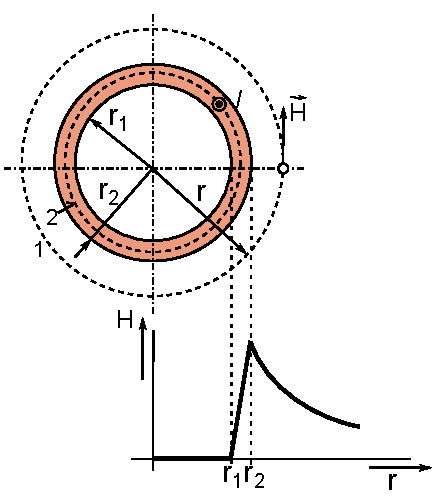
\includegraphics[width=0.8\linewidth]{teo_fig065.pdf}
      \captionof{figure}{K příkladu stanovení intenzity magnetického pole dlouhého dutého válcového 
                vodiče protékaného proudem}
      \label{teo:fig065}
    \par}
    
    Vodič s rovnoměrně rozloženým proudem podle obr. \ref{teo:fig065} je rotačně souměrný podle své
    osy a tedy i jeho magnetické pole je souměrné. Silové čáry jsou soustředné kružnice, vektor
    $\vr{H}$, jenž má směr tečny ke kružnici, je po celé délce kružnice stejně velký. Lze tedy
    snadno použít integrálního tvaru 1. MR (\textbf{zákon celkového proudu})
    
    Pro body ležící vně vodiče obepíná kruhová integrační dráha (vedená po silové čáře 1) celý
    proud vodiče $I$ a platí
    \begin{equation}\label{TEMP:eq_1MR_duty_valec}
      \oint_{\mathcal{C}}\vr{H}d\vr{l} = H\cdot 2\pi r = I
    \end{equation}
    takže intenzita pole je
    \begin{equation}\label{TEMP:eq_H_duty_valec}
      H = \frac{I}{2\pi r}
    \end{equation}
    
    Ve stěně dutého magnetického vodiče jsou silové čáry rovněž kružnice, neboť magnetické pole
    je i zde souměrné. Tyto siločáry však obepínají jen část proudu $I'$ vodiče pro oběh siločáry
    2 platí
    \begin{equation}\label{TEMP:eq_1MR_uvnitr_valce}
      \oint_{\mathcal{C}}\vr{H}d\vr{l} = H\cdot 2\pi r = I' = \pi(r^2-r_1^2)J
    \end{equation}
    kde $J$ je hustota proudu ve vodiči
    \begin{equation}\label{TEMP:eq_J_duty_valec}
      J = \frac{I}{S}= \frac{I}{\pi(r_2^2-r_1^2)}
    \end{equation}
    Ve stěně vodiče je tedy intenzita pole
    \begin{equation}\label{TEMP:eq_H_uvnitr_valce}
      H = \frac{I}{2\pi r}\frac{r^2-r_1^2}{r_2^2-r_1^2}
    \end{equation}
    V dutině vodiče je intenzita rovna nule. Vzhledem k souměrnosti pole by i zde muselo platit
    $\oint_{\mathcal{C}}\vr{H}d\vr{l} = H\cdot 2\pi r$. Protože dráha s poloměrem $r<r_1$ neobepíná
    žádný proud, je $\oint_{\mathcal{C}}\vr{H}d\vr{l} = 0$ a tedy musí byt $H = 0$.
  \end{example}    
\end{mdframed}  
      %------------------------------------------------------------------

      % --------example: $H=f(r)$ souosého kabelu -----------------------
      % \label{TEO:exam013}
      % !TeX spellcheck = cs_CZ
\begin{example}\label{TEMP:ex_koax_H}
  Stanovte intenzitu magnetického pole dlouhého přímého souosého kabelu podle obr.
  \ref{TEMP:fig_exam_koax}. Středním vodičem (\emph{žílou}) prochází proud $I$ a týž proud 
  opačného smyslu prochází vnějším vodičem (\emph{pláštěm}). Proudy jsou rovnoměrně rozloženy po 
  průřezech vodičů. Nakreslete graf průběhu $H = f(r)$ \cite[s.~92]{Dufek1970},
  \cite[s.~195]{Kotlan1999}.
  
  {\centering
   \begin{tabular}{cc}
     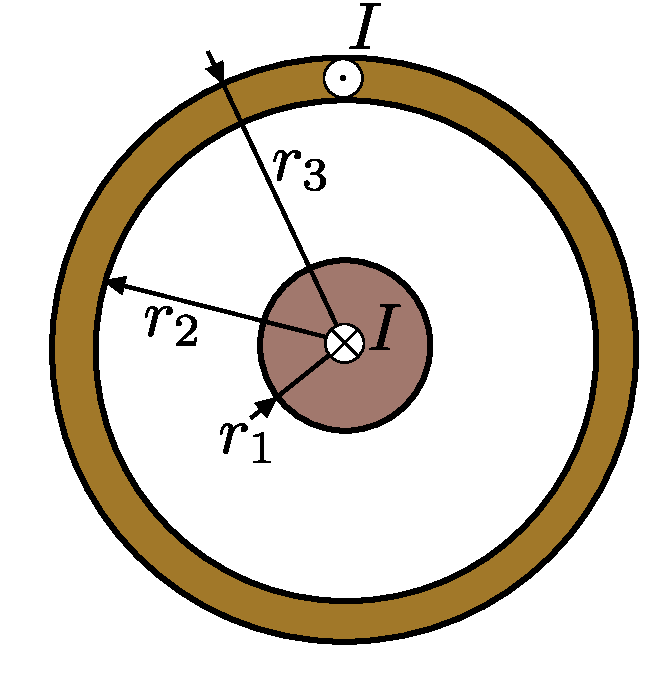
\includegraphics[width=0.4\linewidth]{vypocet_H_sousy_kabel.pdf}   &
     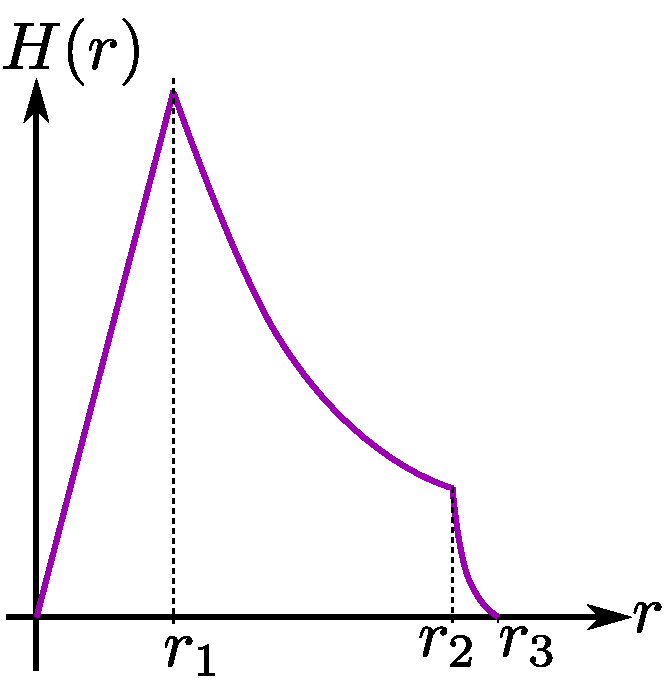
\includegraphics[width=0.4\linewidth]{koax_H_prubeh.pdf}
  \end{tabular}
  \captionsetup{type=figure}
  \captionof{figure}{K příkladu stanovení intenzity magnetického pole dlouhého souosého kabelu 
             protékaného proudem: a) náčrt; b) $H=f(r)$}
  \label{TEMP:fig_exam_koax}
  \par}
  
  \textbf{Řešení}: \newline Rovnici \ref{TEMP:eq_1MR_v_hom_p} aplikujeme na jednotlivé intervaly 
  osově souměrného stacionárního magnetického pole, přičemž se prakticky jedná o superpozici dvou
  polí. V oblasti $r<r_2$ se uplatňuje pouze pole vnitřního válcového vodiče (žíly), pro $r>r_2$ 
  přistupuje souosé pole vnějšího trubkového vodiče.
  \begin{itemize}
    \item Pro oblast $r<r_1$ je vzhledem k 
          \begin{align*}
              % \nonumber to remove numbering (before each equation)
              dI   &= \vr{J}d\vr{S} \\
              I(r) &= \int_S dI = \int_S \vr{J}d\vr{S} = \int_S J\cos\beta dS \\
                   &= \left|\begin{array}{cc}
                               \beta = 0 & H = \text{konst} \\
                             S = \pi r^2 & dS = 2\pi rdr \\
                            \end{array}
                      \right| = J\int_0^r 2\pi rdr = J\pi r^2
          \end{align*}
          hledané řešení 1. MR dáno 
          $$\oint_\mathcal{C}\vr{H}d\vr{l} = H_1 2\pi r = I(r) = J\pi r^2$$ kde celková proudová
          hustota je  $$J = \frac{I}{\pi r_1^2}$$ a tedy $$H_1 = \frac{I}{2\pi r_1^2}\cdot r$$
          
    \item Pro oblast $r_2>r>r_1$ řešíme v podstatě pole vně osamoceného válcového vodiče
          $I(r)$ a tedy $$H_2 = \frac{I}{2\pi r}$$
    \item Pro $r>r_3$ je magnetické pole vytvářeno celým proudem žíly $I$ a příslušnou částí
          proudu pláště $J\pi(r^2 - r_2^2)$, kde proudová hustota $$J =
          \frac{I}{\pi(r_3^2-r_2^2)}$$ má opačnou orientaci oproti proudové hustotě žíly. Pak 
          \begin{align*}
            I(r)                           &= I - I\frac{r^2-r_2^2}{r_3^2-r_2^2} \\
            \oint_\mathcal{C}\vr{H}d\vr{l} &= H_32\pi r = I(r)                   \\          
            H_3                            &= \frac{I}{2\pi r}\left(1 - 
            \frac{r^2 - r_2^2}{r_3^2 - r_2^2}\right) 
          \end{align*}
          Stejný výsledek dostaneme superpozicí opačně orientovaných polí $$H_3 = H'_3 - H''_3 =
          \frac{I}{2\pi r} - \frac{I}{2\pi r}\left(\frac{r^2 - r_2^2}{r_3^2 - r_2^2}\right)$$. 
  \end{itemize}
  Průběh $H(r)$ je na obr. \ref{TEMP:fig_exam_koax}.
\end{example}
  
      %------------------------------------------------------------------

    % -----------Magnetické pole elektrického proudu v diferenciálním tvaru-----------------------
    \subsection{Magnetické pole elektrického proudu v diferenciálním tvaru}
      Nechť je opět magnetické pole vyvoláno konstantním el. proudem $I = \text{konst}$. Jak
      vyplývá z předchozí kapitoly, základním vztahem pro toto pole je \emph{Ampérův zákon}
      $$\oint_{\mathcal{c}}\vec{H_c}\dd{\vec{l}} = I$$  Zvolme za integrační dráhu $c$ obvod malé plošky
      $\Delta S$, jíž prochází proud $\Delta I = J_n \Delta S$, kde $J_n$ je průmět vektoru hustoty
      proudu do směru normály plošky $\Delta S$ (předpokládáme, že ploška $\Delta S$ je dostatečně
      malá, aby se dalo počítat s konstantní hustotou proudu v celém jejím rozsahu)
      \cite[s.~13]{Trnka1972}. Pro zvolený případ platí
      
      \begin{equation}\label{TEMP:eq_amp_z1}
        \oint_{\mathcal{c}}\vec{H_c}\dd{\vec{l}}  =
          J_n \Delta S \rightarrow \frac{1}{\Delta S}\oint_{\mathcal{c}}\vec{H_c}\dd{\vec{l}} = J_n
      \end{equation} 
      
      Pro $\Delta S \rightarrow 0$ zavedeme označení 
      \begin{equation}\label{TEMP:eq_amp_z2}
        \rot{H}  = \frac{1}{\Delta S}\oint_{\mathcal{c}}\vec{H_c}\dd{\vec{l}}  = J_n
      \end{equation}
      
      Rovnice \ref{TEMP:eq_amp_z2} říká, že \emph{rotace vektoru} $\vec{H}$, ($\rot{H}$), jehož
      průmět do určitého směru je roven průmětu vektoru hustoty proudu do tohoto směřu. Z uvedených
      vztahu je patrný fyzikální význam rotace vektoru $\vec{H}$. Je to vektor, jehož velikost je
      rovna oběhovému magnetickému napětí po dráze v rovině kolmé k vektoru hustoty proudu,
      vztaženém k ploše obepínané oběhovou drahou (v nehomogenní poli to platí pro případ, že se
      plocha dráhy blíží k nule).
      
      Při použití pravoúhlé soustavy kartézských souřadnic \(x\), \(y\) a $z$ jsou průměty vektoru
      $\rot{H}$ do jednotlivých os
      \begin{equation}\label{TEMP:eq_amp_z3}
        \textsf{rot}_x\vec{H} = J_x,   \quad
        \textsf{rot}_y\vec{H} = J_y,   \quad
        \textsf{rot}_z\vec{H} = J_z    
      \end{equation}      
      Průmět $\textsf{rot}_x\vec{H}$ je dán oběhovým magnetickým napětím po obvodu plošky
      \(\dd{y}\dd{z}\) a platí
      \begin{align*}
        \textsf{rot}_x\vec{H} 
        &=\frac{1}{\dd{y}\dd{z}}\oint_{\mathcal{c}}\vec{H_c}\dd{\vec{l}} =               \nonumber\\
        &=\frac{1}{\dd{y}\dd{z}}\cdot\Biggl[\Biggr.\left[H_y\dd{y} 
         +\left(H_z + \pder{Hz}{y}\dd{y}\right)\dd{z}\right]                             \nonumber\\     
        &-\left[\left(H_y-\pder{H_y}{z}\dd{z}\right)\dd{y}-H_z\dd{z}\right]\Biggl.\Biggr]\nonumber\\
        &=\pder{H_z}{y}\dd{y}\dd{z} - \pder{H_y}{z}\dd{y}\dd{z}                          \nonumber\\    
        &=\pder{H_z}{y} - \pder{H_y}{z} = J_z
      \end{align*}       
      
      \luagraphic[0.8]{teo_fig062.pdf}{K odvození pojmu \(\textsf{rot}_z\vec{H}\)}{teo:fig062}
         
      tedy dostáváme
      \begin{subequations}
        \begin{align}\label{TEMP:eq_amp_z5}
          \textsf{rot}_x\vec{H} &= \pder{H_z}{y} - \pder{H_y}{z} = J_x       \\
          \textsf{rot}_y\vec{H} &= \pder{H_x}{z} - \pder{H_z}{x} = J_y       \\
          \textsf{rot}_z\vec{H} &= \pder{H_y}{x} - \pder{H_x}{y} = J_z            
        \end{align}    
    \end{subequations}    
      Pro \emph{pravoúhlé souřadnice} $x, y, z$ můžeme tedy vztah $\rot{H} = \vec{J}$ rozepsat na
      tvar
      \begin{align*}
        \textsf{rot}\vec{H} 
          &= \vec{i}\,\textsf{rot}_x\vec{H} + 
             \vec{j}\,\textsf{rot}_y\vec{H} +
             \vec{k}\,\textsf{rot}_z\vec{H}                                    \\
          &= \vec{i}\left(\pder{H_z}{y} - \pder{H_y}{z}\right) +               \\
          &+ \vec{j}\left(\pder{H_x}{z} - \pder{H_z}{x}\right) +               \\
          &+ \vec{k}\left(\pder{H_y}{x} - \pder{H_x}{y}\right)                 \\  
          &= \vec{i}\,J_x + \vec{j}\,J_y + \vec{k}\,J_z = \vec{J}.
      \end{align*}          
      
      Rotaci vektoru $\rot{H}$ můžeme též symbolicky vyjádřit vektorovým součinem Hamiltonova
      operátoru a vektoru $\vec{H}$
      \begin{align*}
        \rot{H} &= \nabla\times\vec{H}                                                      \\                                           
                &= \left(\vec{i}\,\pder{ }{x} + 
                   \vec{j}\,\pder{ }{y} + \vec{k}\,\pder{ }{z}\right)                       \\
                & \times(\vec{i}\,H_x + \vec{j}\,H_y + \vec{k}\,H_z)
      \end{align*}
      nebo také determinantu
      \begin{equation}\label{TEMP:eq_amp_z8}
        \rot{H} = \begin{vmatrix}
                    \vec{i}       & \vec{j}      & \vec{k}      \\
                    \pder{ }{x}  & \pder{ }{y} & \pder{ }{z} \\ 
                    H_x          & H_y         & H_z         \\
                  \end{vmatrix}      
      \end{equation}  
      \emph{cylindrických souřadnic} $r$, $\varphi$, $z$:
      \begin{align}\label{TEMP:eq_amp_z9}
        \textsf{rot}_r\vec{H}       
          &= \frac{1}{r}\pder{H_z}{\varphi} - \pder{H_\varphi}{z} = J_r           \nonumber \\ 
        \textsf{rot}_\varphi\vec{H} 
          &= \pder{H_r}{z} - \pder{H_z}{r}                        = J_\varphi     \nonumber \\
        \textsf{rot}_z\vec{H}       
          &= \frac{1}{r}\left[\pder{ }{r}
             \left(rH_\varphi\right)-\pder{H_r}{\varphi}\right]   = J_z
      \end{align} 
      \emph{sférických souřadnic} $r$, $\varphi$, $\vartheta$ 
      \begin{align}\label{TEMP:eq_amp_z10}
        \textsf{rot}_r\vec{H}        
           &= \frac{1}{r\sin\vartheta}\left[\pder{ }{\vartheta}(H_\varphi\sin\vartheta) - 
              \pder{H_\vartheta}{\varphi}\right]                     = J_r           \nonumber \\ 
        \textsf{rot}_\varphi\vec{H}   
           &= \frac{1}{r}\left[\pder{ }{r}(rH_\vartheta) - 
              \pder{H_r}{\vartheta}\right]                           = J_\varphi     \nonumber \\
        \textsf{rot}_\vartheta\vec{H} 
           &= \frac{1}{r\sin\vartheta}\left[\pder{H_r}{\varphi} -
              \pder{ }{r}\left(rH_\varphi\sin\vartheta\right)\right] = J_\vartheta    
    \end{align} 
      Podobně jako v elektrickém poli vyjadřujeme vztah $\oint\vec{D}\dd{\vec{S}} = Q$ vztahem 
      $\diver{D}
      = \rho$, tak i v magnetickém poli vyjadřujeme vztah $\oint\vec{B}\dd{\vec{S}} = 0$ vztahem
      $\diver{D} = 0$, nebo též v kartézských souřadnicích \(x\), \(y\) a $z$ jako $$\diver{D} =
      \nabla\cdot\vec{B} = \pder{B_x}{x} + \pder{B_y}{y} + \pder{B_z}{z} = 0$$
                     
    % ----------------Rovnice pro magnetický potenciál -------------------------------------------
    \subsection{Rovnice pro magnetický potenciál}
      V regulárních bodech lineárního homogenního izotropního magnetika platí pro $\varphi_m$
      \textbf{Laplaceova rovnice}
      \begin{equation}\label{TEMP:eq_varphi_m_laplace}
        \Delta\varphi_m = 0
      \end{equation}      
      Důkaz plyne z rovnice $\diver{B} = 0$ a rovnice $\vec{B} = \mu\vec{H}$: $$\diver{B} =
      \textsf{div}\mu\vec{H} = \textsf{div}\mu(-\textsf{grad}\varphi_m).$$ Pro $\mu = \text{konst}$
      dostáváme $\textsf{div}\textsf{grad}\varphi_m = 0$, což je rovnice
      \ref{TEMP:eq_varphi_m_laplace}.
      
      Na rozhraní mezi dvěma magneticky různými prostředími neplatí Maxwellovy rovnice v
      diferenciálním tvaru a tedy ani Laplaceova rovnice \ref{TEMP:eq_varphi_m_laplace}. Podmínky 
      pro $\vec{H}$ a $\vec{B}$ na rozhraní vyjádříme pomocí skalárního magnetického potenciálu
       \begin{align}\label{TEMP:eq_mag_U_rozhrani}
         \varphi_{m1}                 &= \varphi_{m2} \\
         \mu_1\pder{\varphi_{m1}}{n}  &= \mu_2\pder{\varphi_{m2}}{n} 
       \end{align}
      kde $\pder{}{n}$ jsou derivace ve směru normály k rozhraní. 
    
    \subsubsection{Vektorový magnetický potenciál}
      V elektrostatice jsme pro usnadnění mnohých problémů zavedli skalární elektrický potenciál -
      lze jej zavést vždy, neboť elektrostatické pole je vždy potenciální. Magnetické pole je však
      obecně vírové. Lze jej popsat skalárním potenciálem jen ve speciálních případech, tj.
      jestliže je polem potenciálním. Obecně je však zavedení skalárního potenciálu nepřípustné.
      Lze i pak zavést nějakou veličinu (analogickou skalárnímu potenciálu), s níž by se pracovalo
      snáze, než přímo s vektory pole?
      
      Dříve než definujeme vektorový magnetický potenciál, zopakujme zavedení skalárního potenciálu
      v elektrostatice. Vyjdeme z 2. MR a z rovnice známé z vektorové analýzy: $$\rot{E} = 0 \quad
      \text{a} \quad \textsf{rot}\,\textsf{grad}\varphi_m = 0.$$
      
      V magnetickém poli vyjdeme ze 4. MR a z jiné identity pro vektorovou funkci $\vec{A}$, známe z
      vektorové analýzy: $$\diver{B} = 0 \quad \text{a} \quad \textsf{div}\textsf{rot}\vec{A} =
      0$$ odtud
        \begin{equation}\label{TEMP:eq_B_rotA}
          \vec{B} = \rot{A}.
        \end{equation}       
               
%} % tikzset
%~~~~~~~~~~~~~~~~~~~~~~~~~~~~~~~~~~~~~~~~~~~~~~~~~~~~~~~~~~~~~~~~~~~~~~~~~~~~~~~~~~~~~~~~~~~~~~~~~~